\documentclass[12pt]{article}

% taken from APL Memo style
\topmargin      -1in 
\marginparsep   0in
\headheight     .75in  
\headsep        0.25in
\textheight     9in 
\oddsidemargin  0in 
\evensidemargin 0in 
\textwidth      6.50in 

\pdfoptionpdfminorversion=6

\usepackage[hyphens]{url}
\usepackage{hyperref}
\usepackage{subcaption}
\usepackage{fancyhdr}
\usepackage[usenames,dvipsnames]{color}
\usepackage{listings}  
\usepackage{cite}
\usepackage{graphicx}
\usepackage{mathptmx}
\usepackage{acronym}
\usepackage{array}
\usepackage{gensymb}
\usepackage[toc,page]{appendix}
\usepackage{color, colortbl}
\usepackage{multirow}
\usepackage{booktabs}
\usepackage{gensymb}
\usepackage[nottoc]{tocbibind}

\definecolor{Gray}{gray}{0.9}

\newcolumntype{L}{>{\centering\arraybackslash}m{3cm}}
\hypersetup{colorlinks=true, 
	 	    linkcolor=black, 
		    urlcolor=black, 
		    citecolor=black,
		    filecolor=black}
		    
\urlstyle{rm}

% add any other paths here where images might reside (ideally a relative path)
\graphicspath{ {images/} }

% for two-column references
% from: http://tex.stackexchange.com/questions/20758/bibliography-in-two-columns-section-title-in-one
%\usepackage{multicol}
%\usepackage{etoolbox}
%\patchcmd{\thebibliography}{\section*{\refname}}
%    {\begin{multicols}{2}[\section*{\refname}]}{}{}
%\patchcmd{\endthebibliography}{\endlist}{\endlist\end{multicols}}{}{}
\setlength{\parindent}{0in}

\acrodef{nlp}[NLP]{Natural Language Processing}
\acrodef{bow}[BOW]{Bag of Words}
\acrodef{cnn}[CNN]{Convolutional Neural Network}
%%% paragraph spacing
%\setlength{\parindent}{4em}
\setlength{\parskip}{1em}

\begin{document}
\begin{titlepage}
	\centering
	
\includegraphics[width=\textwidth]{jhu_logo.png}\par\vspace{2cm}
	{\scshape\Huge Application of Convolutional Neural Networks to Natural Language Processing \\
	\vspace{1.5cm}
	 \scshape\Large EN.525.801(21) - Special Project I Summer 2016\par}
	{\scshape \Large Austin Dress\par} 
	\vspace{0.75cm}
%	{\scshape \Large DRAFT\par}
	\vfill
	{\large \today\par}
\end{titlepage}

\tableofcontents
\listoftables

\newpage

\section{Preface} 
\ac{nlp} is a field in computer science that focuses on processing human language. Human language can be referred to as a natural language as it has evolved overtime without strict syntax rules that one would find in programming languages. A simple example of \ac{nlp} would be processing a sentence and identifying the verb, subject, adjective. Writing a program to process a scholarly article and generate a summary would be a more advanced application of \ac{nlp}.

In recent years \ac{cnn}s, a deep learning technique for image classification, have gained huge popularity after Alex Krizhevsky won the Imagenet LSVRC2012 competition with his network \cite{alex}.

\section{Development Schedule}

In Figure \ref{fig:schedule} the development schedule is shown for the project. Past, present, and future events are shown on this schedule. At time of submitting this CDR document it will be February 29th. At this point the project is in development. 

\begin{figure}[htbp]
  \centering
  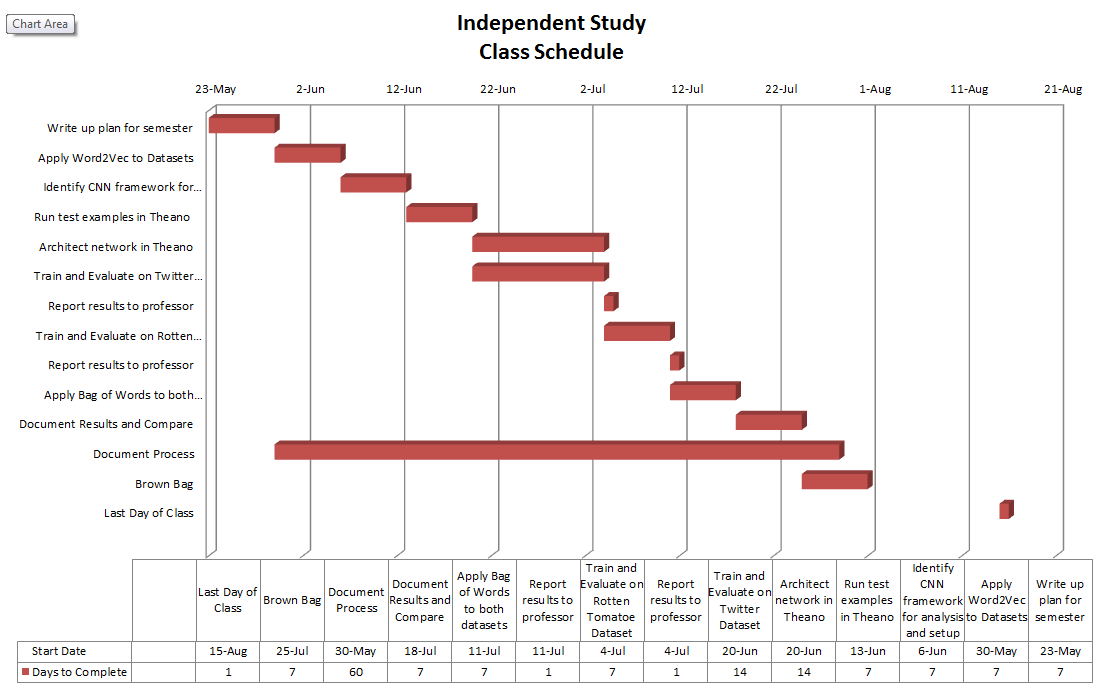
\includegraphics[scale=.5]{gantt.PNG}
  \caption{Project Development Schedule}
  \label{fig:schedule}
\end{figure}


\newpage
\bibliography{Austin_Dress_NLP_CNN_Summer_2016.bib}
\bibliographystyle{plain}

\end{document}
